\section{Datos obtenidos: discusión y cálculo de errores}

A continuación se presentan los datos relevados para cada componente y sus respectivas curvas características $I=f(V)$. 

\subsection{Resistor de Carbón Depositado}

El resistor ensayado tenía un valor nominal de $R_{nom} = \SI{220}{\ohm}$ con una tolerancia del 5\% (asumida por el código de colores). Al medirlo con el multímetro, se obtuvo un valor estático de $R_{med} = \SI{216}{\ohm}$.

Luego, los datos experimentales de tensión y corriente se tabularon (Tabla \ref{tab:res_220} del Anexo) y graficaron, mostrando un comportamiento lineal típico de un dispositivo óhmico (Figura \ref{fig:curva_resistor}).


\begin{figure}[H]
    \centering
    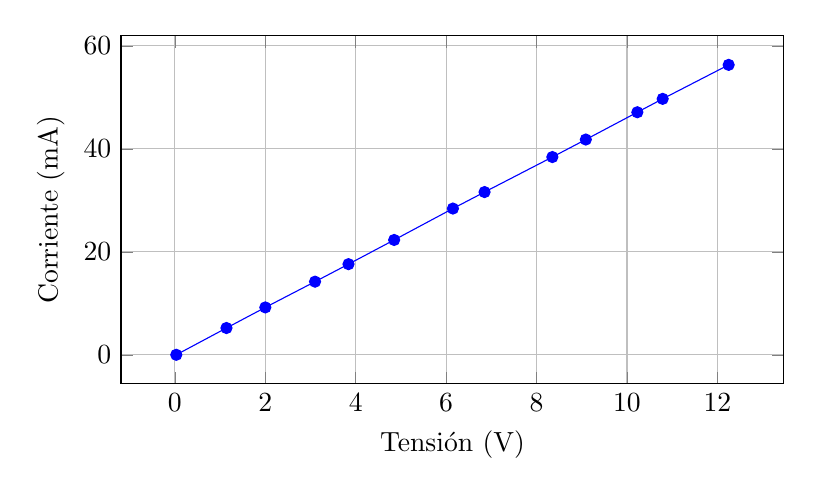
\begin{tikzpicture}
        \begin{axis}[
            width=10cm, height=6cm,
            xlabel={Tensión (V)}, ylabel={Corriente (mA)},
            grid=major,
            legend pos=north west
        ]
        \addplot[color=blue, mark=*] coordinates {
            (0.03,0) (1.14,5.2) (2.0,9.2) (3.1,14.2) (3.84,17.6) 
            (4.85,22.3) (6.15,28.4) (6.85,31.6) (8.35,38.4) (9.09,41.8) 
            (10.23,47.1) (10.79,49.7) (12.25,56.3)
        };
        \end{axis}
    \end{tikzpicture}
    \caption{Curva característica del resistor de carbón.}
    \label{fig:curva_resistor}
\end{figure}

\textbf{Cálculo de error:}
Calculando la resistencia dinámica (pendiente de la recta) tomando los puntos extremos, se obtuvo $R_{din} = \frac{\Delta V}{\Delta I} = \frac{12.25\text{ V} - 0.03\text{ V}}{56.3\text{ mA} - 0\text{ mA}} \approx \SI{217.05}{\ohm}$. 
El error relativo porcentual respecto al valor medido con el multímetro ($\SI{216}{\ohm}$) fue:
\begin{equation}
    e\% = \left| \frac{216 - 217.05}{216} \right| \cdot 100 \approx 0.49\%
\end{equation}
Esto demuestra una excelente concordancia y confirma el comportamiento lineal.

\vspace{0.5cm}

\subsection{Lámpara de Filamento de Tungsteno}

En la Tabla \ref{tab:lampara} del Anexo se presentan los valores obtenidos durante el aumento de la tensión aplicada a la lámpara. El resultado gráfico se presenta en la Figura \ref{fig:curva_lampara} para mostrar la evolución completa de la curva característica.

\begin{figure}[H]
    \centering
    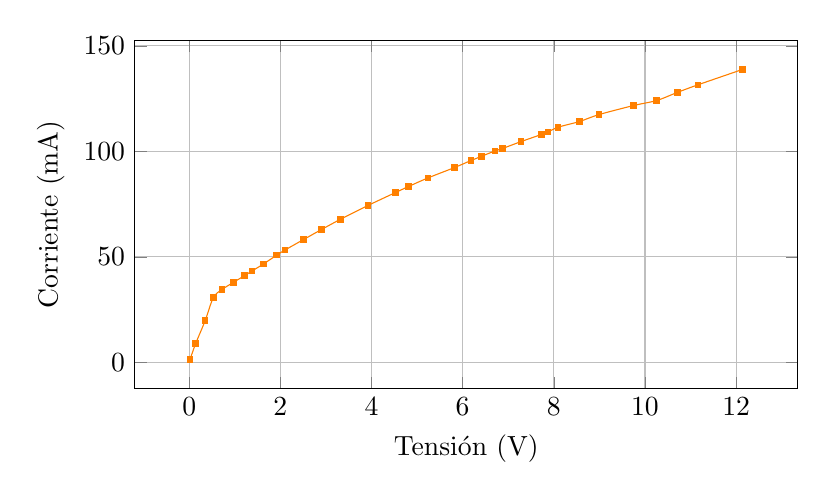
\begin{tikzpicture}
        \begin{axis}[
            width=10cm, height=6cm,
            xlabel={Tensión (V)}, ylabel={Corriente (mA)},
            grid=major, smooth
        ]
        \addplot[color=orange, mark=square*, mark size=1pt] coordinates {
            (0.02, 1.4) (0.14, 8.8) (0.35, 19.7) (0.53, 30.7) (0.72, 34.5)
            (0.97, 37.9) (1.21, 41.0) (1.38, 43.3) (1.63, 46.6) (1.92, 50.8)
            (2.10, 53.2) (2.51, 58.2) (2.90, 62.9) (3.32, 67.8) (3.92, 74.3)
            (4.53, 80.5) (4.81, 83.3) (5.24, 87.4) (5.82, 92.3) (6.18, 95.6)
            (6.41, 97.6) (6.71, 100.2) (6.87, 101.3) (7.28, 104.6) (7.73, 108.0)
            (7.87, 109.1) (8.09, 111.4) (8.56, 114.1) (8.99, 117.4) (9.75, 121.7)
            (10.26, 124.1) (10.72, 128.0) (11.16, 131.5) (12.14, 138.8)
        };
        \end{axis}
    \end{tikzpicture}
    \caption{Curva característica de la lámpara de tungsteno.}
    \label{fig:curva_lampara}
\end{figure}

\textbf{Análisis de la Resistencia Térmica en la Lámpara}: 
Por otro lado, para cada valor de V e I se calculó la resistencia estática asociada $R = V/I$ para comprobar el Efecto Joule. Los resultados se presentan en la Figura \ref{fig:curva_resistencia_lampara} a continuación.

\begin{figure}[H]
    \centering
    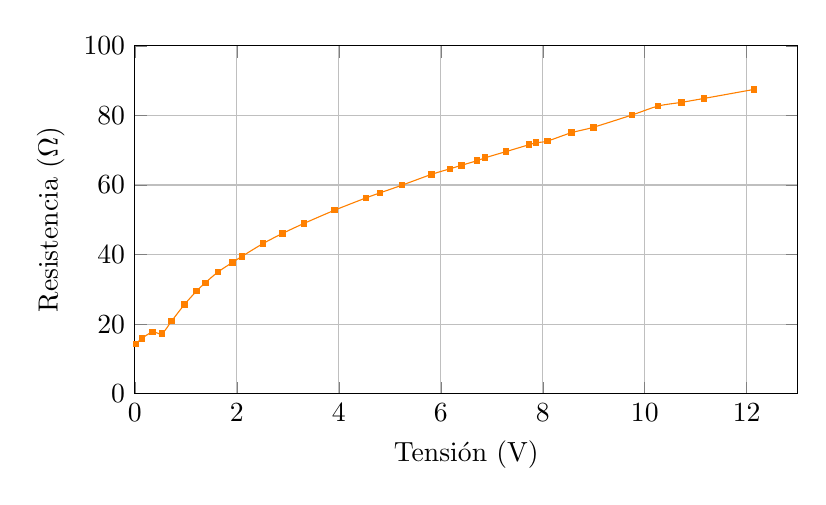
\begin{tikzpicture}
        \begin{axis}[
            width=10cm, height=6cm,
            xlabel={Tensión (V)}, ylabel={Resistencia ($\Omega$)},
            grid=major, smooth,
            xmin=0, xmax=13,
            ymin=0, ymax=100
        ]
        \addplot[color=orange, mark=square*, mark size=1pt] coordinates {
            (0.02,14.29) (0.14,15.91) (0.35,17.77) (0.53,17.26) (0.72,20.87) 
            (0.97,25.59) (1.21,29.51) (1.38,31.87) (1.63,34.98) (1.92,37.80) 
            (2.1,39.47) (2.51,43.13) (2.9,46.10) (3.32,48.97) (3.92,52.76) 
            (4.53,56.27) (4.81,57.74) (5.24,59.95) (5.82,63.06) (6.18,64.64) 
            (6.41,65.68) (6.71,66.97) (6.87,67.82) (7.28,69.60) (7.73,71.57) 
            (7.87,72.14) (8.09,72.62) (8.56,75.02) (8.99,76.58) (9.75,80.12) 
            (10.26,82.68) (10.72,83.75) (11.16,84.87) (12.14,87.46)
        };
        \end{axis}
    \end{tikzpicture}
    \caption{Variación de la resistencia asociada del filamento en función de la tensión aplicada.}
    \label{fig:curva_resistencia_lampara}
\end{figure}

\vspace{0.5cm}

\subsection{Diodos (Silicio y LED)}

Para los componentes semiconductores, se tabularon los valores que evidencian la tensión de umbral donde comienza la conducción abrupta (Tablas \ref{tab:led_res} y \ref{tab:diodo} del Anexo). Se presentan ambas mediciones completas gráficamente para su posterior comparación (Figuras \ref{fig:curva_diodo} y \ref{fig:curva_led}). 

\begin{figure}[H]
    \centering
    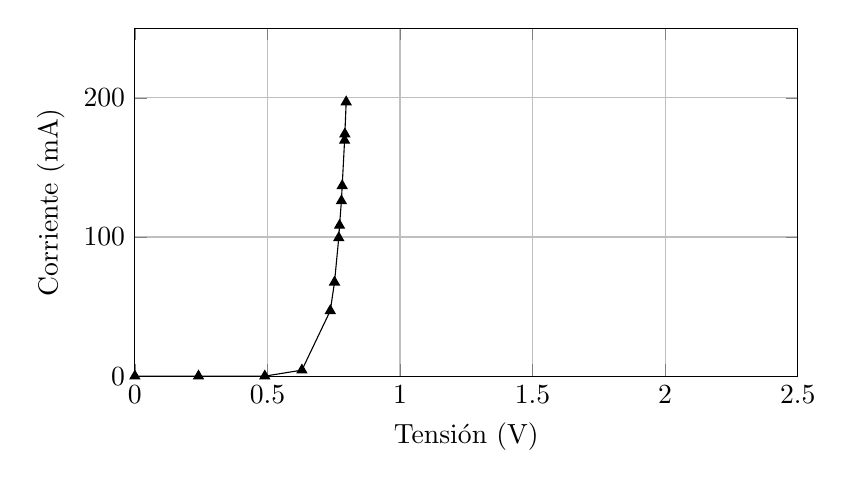
\begin{tikzpicture}
        \begin{axis}[
            width=10cm, height=6cm,
            xlabel={Tensión (V)}, ylabel={Corriente (mA)},
            grid=major,
            legend pos=north east,
            xmin=0, xmax=2.5,
            ymin=0, ymax=250
        ]
        % Diodo Silicio
        \addplot[color=black, mark=triangle*, mark size=2pt] coordinates {
            (0.0,0.0) (0.24,0.0) (0.49,0.0) (0.63,4.3) (0.737,47.0) 
            (0.753,67.5) (0.769,99.4) (0.772,108.3) (0.779,125.9) 
            (0.782,136.8) (0.791,169.4) (0.792,174) (0.797,197)
        };
        \end{axis}
    \end{tikzpicture}
    \caption{Curva característica del diodo de silicio.}
    \label{fig:curva_diodo}
\end{figure}

\begin{figure}[H]
    \centering
    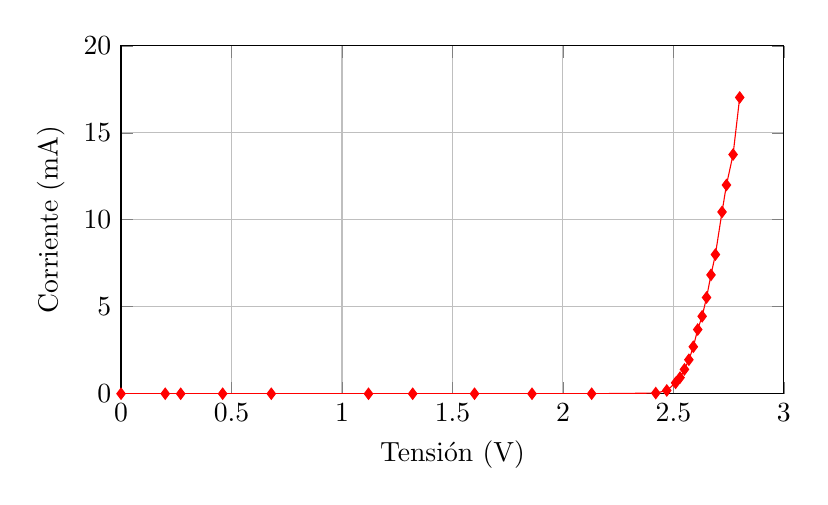
\begin{tikzpicture}
        \begin{axis}[
            width=10cm, height=6cm,
            xlabel={Tensión (V)}, ylabel={Corriente (mA)},
            grid=major,
            legend pos=north east,
            xmin=0, xmax=3,
            ymin=0, ymax=20
        ]        
        % LED Rojo
        \addplot[color=red, mark=diamond*, mark size=2pt] coordinates {
            (0,0) (0.2,0) (0.27,0) (0.46,0) (0.68,0) 
            (1.12,0) (1.32,0) (1.6,0) (1.86,0) (2.13,0) 
            (2.42,0.035) (2.47,0.186) (2.51,0.625) (2.53,0.924) (2.55,1.399) 
            (2.57,1.952) (2.59,2.7) (2.61,3.69) (2.63,4.45) (2.65,5.53) 
            (2.67,6.83) (2.69,8) (2.72,10.45) (2.74,12) (2.77,13.75) 
            (2.8,17.03)
        };
        \end{axis}
    \end{tikzpicture}
    \caption{Curva característica del LED rojo.}
    \label{fig:curva_led}
\end{figure}

\textbf{Análisis Logarítmico del Diodo (Ecuación de Shockley)}: 
Para verificar el comportamiento exponencial predicho por la ecuación ideal del diodo (Ecuacion \ref{eq:shockley}), se procedió a linealizar la curva aplicando el logaritmo a la corriente medida.

Los valores nulos de corriente fueron descartados del análisis, graficando únicamente los puntos pertenecientes a la zona de conducción directa. Se puede apreciar el resultado en las siguientes figuras (\ref{fig:log_diodo_si} y \ref{fig:log_led_rojo}), donde se observa un comportamiento lineal para ambos dispositivos.

\begin{figure}[htbp]
    \centering
    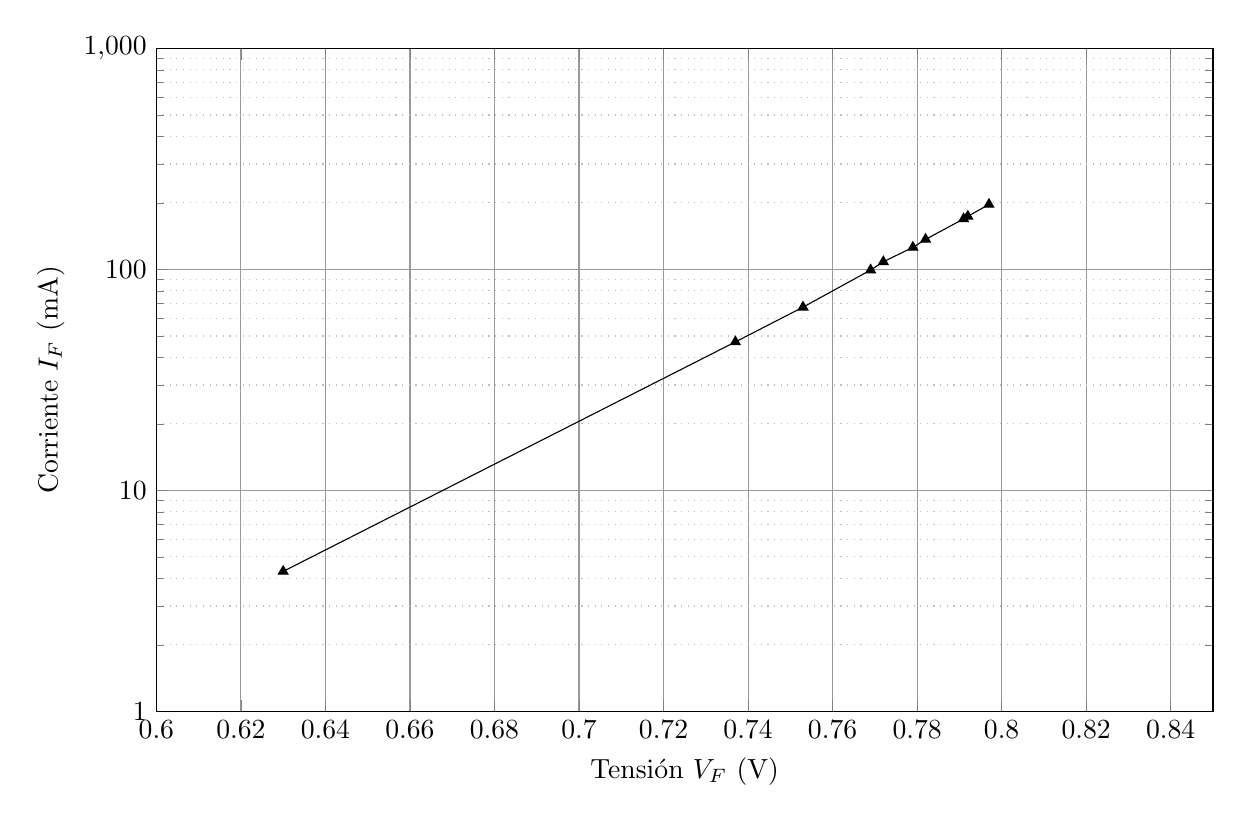
\begin{tikzpicture}
        \begin{semilogyaxis}[
            width=15cm, height=10cm,
            xlabel={Tensión $V_F$ (V)},
            ylabel={Corriente $I_F$ (mA)},
            grid=both,
            minor grid style={dotted, gray!50},
            major grid style={gray!80},
            xmin=0.6, xmax=0.85, % Zoom en la zona de conducción del Si
            ymin=1, ymax=1000,
            log ticks with fixed point,
            ytick={1, 10, 100, 1000},
        ]
        \addplot[color=black, mark=triangle*, mark size=2pt] coordinates {
            (0.63,4.3) (0.737,47.0) 
            (0.753,67.5) (0.769,99.4) (0.772,108.3) (0.779,125.9) 
            (0.782,136.8) (0.791,169.4) (0.792,174) (0.797,197)
        };
        \end{semilogyaxis}
    \end{tikzpicture}
    \caption{Curva característica semilogarítmica de tensión-corriente para un diodo de silicio en polarización directa.}
    \label{fig:log_diodo_si}
\end{figure}

\begin{figure}[htbp]
    \centering
    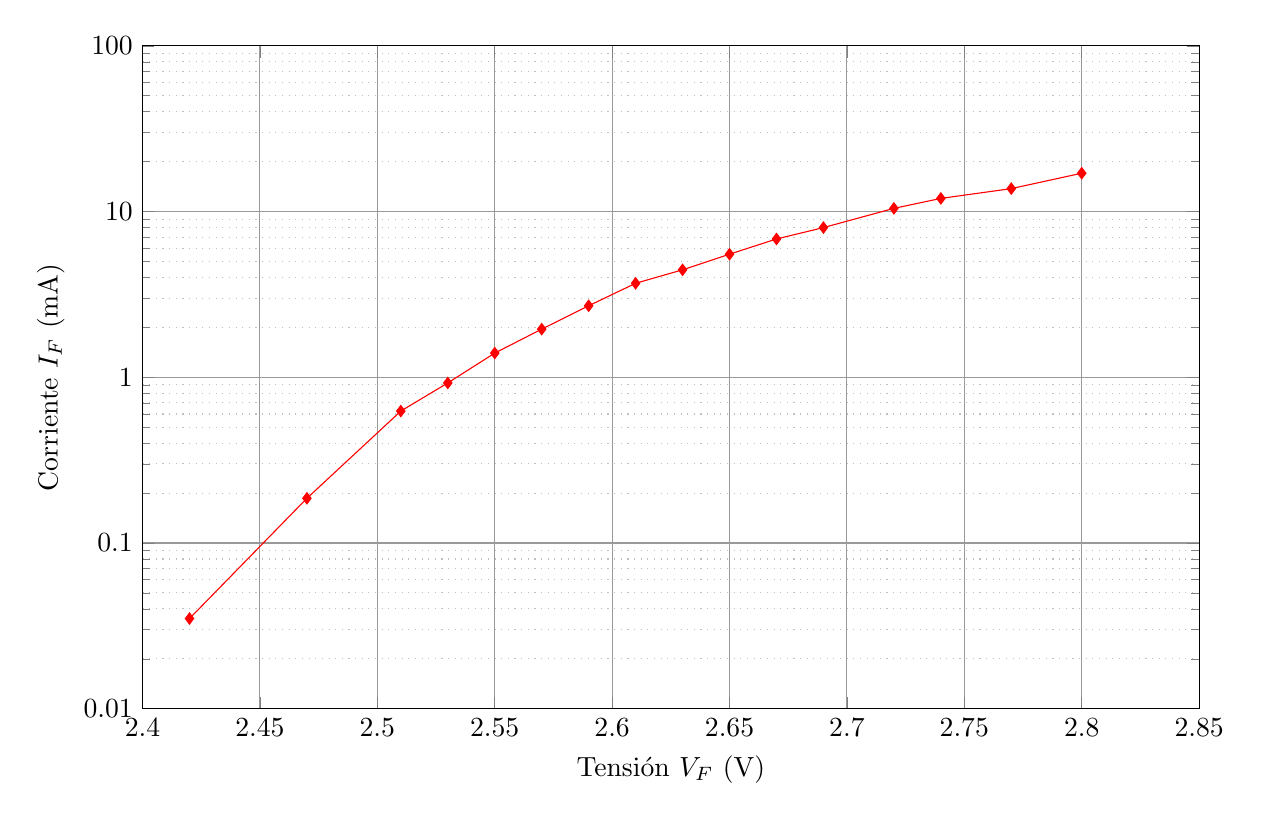
\begin{tikzpicture}
        \begin{semilogyaxis}[
            width=15cm, height=10cm,
            xlabel={Tensión $V_F$ (V)},
            ylabel={Corriente $I_F$ (mA)},
            grid=both,
            minor grid style={dotted, gray!50},
            major grid style={gray!80},
            xmin=2.4, xmax=2.85,
            ymin=0.01, ymax=100,
            log ticks with fixed point,
            ytick={0.01, 0.1, 1, 10, 100},
        ]
        \addplot[color=red, mark=diamond*, mark size=2pt] coordinates {            
            (2.42,0.035) (2.47,0.186) (2.51,0.625) (2.53,0.924) (2.55,1.399) 
            (2.57,1.952) (2.59,2.7) (2.61,3.69) (2.63,4.45) (2.65,5.53) 
            (2.67,6.83) (2.69,8) (2.72,10.45) (2.74,12) (2.77,13.75) 
            (2.8,17.03)
        };
        \end{semilogyaxis}
    \end{tikzpicture}
    \caption{Curva característica semilogarítmica de tensión-corriente para un diodo LED rojo en polarización directa.}
    \label{fig:log_led_rojo}
\end{figure}